\documentclass[aspectratio=169]{beamer}

\usepackage[utf8]{inputenc}
\usepackage{graphicx}
\usepackage{tikz}
\usetikzlibrary{positioning,patterns,arrows.meta}
\usepackage[export]{adjustbox}
\usepackage{pifont}

\usefonttheme{professionalfonts}

% Theme
\usetheme{Madrid}
\definecolor{ucdgreen}{RGB}{0, 102, 51}
\definecolor{gapred}{RGB}{180, 50, 50}
\definecolor{vennblue}{RGB}{70, 130, 180}
\definecolor{vennorange}{RGB}{210, 140, 50}
\usecolortheme[named=ucdgreen]{structure}
\setbeamertemplate{navigation symbols}{}

% Title metadata
\title[Multi-Hazard S2S Predictability]{Multi-Hazard Predictability at Subseasonal Timescales}
\author[Lainey Ward]{Lainey Ward}
\institute[]{Decarb-AI Centre, School of Civil Engineering\\
Primary supervisor: Dr Fiachra O'Loughlin \\ Co-supervisor: Dr Conor Sweeney}
\date{}

\begin{document}

% Title slide
\begin{frame}
  \titlepage
\end{frame}

% --------------------------------------------------
% SLIDE 1: Opening — The prediction gap
% --------------------------------------------------
\begin{frame}{The Prediction Gap}

    \begin{columns}[c,totalwidth=\textwidth]

        \begin{column}{0.55\textwidth}
            \centering
            \includegraphics[width=\textwidth]{s2s.png}

            \vspace{0.3em}
            {\tiny Source: Seasoned Chaos}
        \end{column}

        \begin{column}{0.43\textwidth}
            \centering
            \vspace{1em}
            {\Large\textbf{2 weeks -- 2 months}}

            \vspace{1.5em}
            Least skilful\\[0.5em]
            Most decision-relevant
        \end{column}

    \end{columns}
\end{frame}

% --------------------------------------------------
% SLIDE 2: How do we currently forecast at S2S?
% --------------------------------------------------
\begin{frame}{How Do We Forecast at S2S Timescales?}

    \centering
    \vspace{0.5em}
    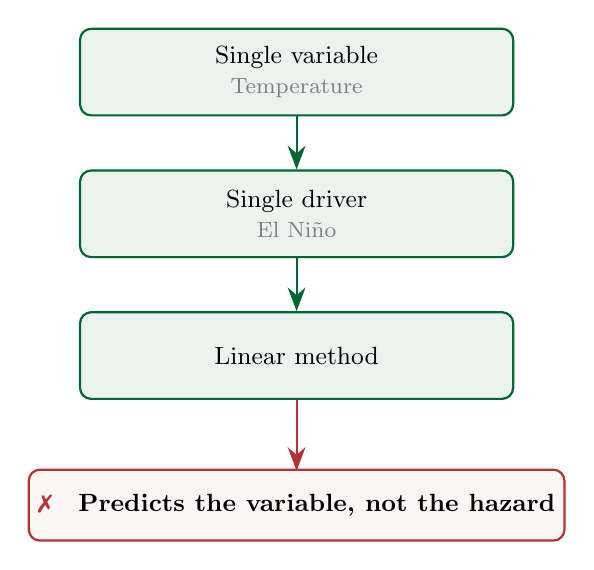
\begin{tikzpicture}[
        pbox/.style={draw=ucdgreen, thick, rounded corners,
                    minimum width=5.5cm, minimum height=1.1cm,
                    fill=ucdgreen!8, align=center},
        crit/.style={draw=gapred, thick, rounded corners,
                    minimum width=5.5cm, minimum height=0.9cm,
                    fill=gapred!5, align=center, font=\small\bfseries},
        arr/.style={-{Stealth[length=3mm]}, thick, ucdgreen}
    ]
    % Step 1: pick a single variable
    \onslide<2->{
    \node[pbox] (var) at (0, 3.6)
         {\small Single variable\\[-0.1em]{\footnotesize\color{gray} Temperature}};
    }
    % Step 2: condition on one driver
    \onslide<3->{
    \node[pbox] (drv) at (0, 1.8)
         {\small Single driver\\[-0.1em]{\footnotesize\color{gray} El Ni\~no}};
    \draw[arr] (var) -- (drv);
    }
    % Step 3: linear method
    \onslide<4->{
    \node[pbox] (skl) at (0, 0)
         {\small Linear method};
    \draw[arr] (drv) -- (skl);
    }

    % Critique endpoint
    \onslide<5->{
    \draw[-{Stealth[length=3mm]}, thick, gapred] (skl.south) -- ++(0,-0.9);
    \node[crit] at (0, -1.9)
         {{\color{gapred}\ding{55}}\;\; Predicts the variable, not the hazard};
    }
    \end{tikzpicture}
\end{frame}

% --------------------------------------------------
% SLIDE 3: Why does this approach fail for multi-hazards?
% --------------------------------------------------
\begin{frame}{Why Does This Approach Fail?}

    \centering
    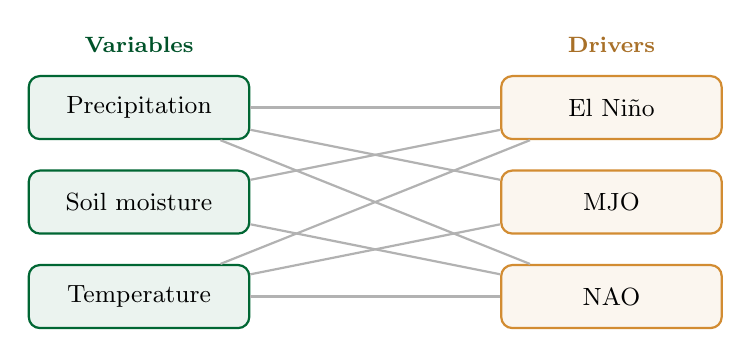
\begin{tikzpicture}[
        vbox/.style={draw=ucdgreen, thick, rounded corners,
                    minimum width=2.8cm, minimum height=0.8cm,
                    fill=ucdgreen!8, align=center, font=\small},
        dbox/.style={draw=vennorange, thick, rounded corners,
                    minimum width=2.8cm, minimum height=0.8cm,
                    fill=vennorange!8, align=center, font=\small},
        link/.style={-, thick, gray!60}
    ]
    % Column label
    \node[font=\footnotesize\bfseries, text=ucdgreen!80!black] at (-3, 3.2) {Variables};
    \node[font=\footnotesize\bfseries, text=vennorange!80!black] at (3, 3.2) {Drivers};

    % Left column — variables
    \node[vbox] (precip) at (-3, 2.4) {Precipitation};
    \node[vbox] (soil)   at (-3, 1.2) {Soil moisture};
    \node[vbox] (temp)   at (-3, 0)   {Temperature};

    % Right column — drivers
    \node[dbox] (enso) at (3, 2.4) {El Ni\~no};
    \node[dbox] (mjo)  at (3, 1.2) {MJO};
    \node[dbox] (nao)  at (3, 0)   {NAO};

    % Criss-crossing connections
    \draw[link] (enso) -- (precip);
    \draw[link] (enso) -- (temp);
    \draw[link] (enso) -- (soil);
    \draw[link] (mjo)  -- (precip);
    \draw[link] (mjo)  -- (temp);
    \draw[link] (nao)  -- (precip);
    \draw[link] (nao)  -- (temp);
    \draw[link] (nao)  -- (soil);

    \end{tikzpicture}
\end{frame}

% --------------------------------------------------
% SLIDE 4: Q3 — Can we close this gap?
% --------------------------------------------------
\begin{frame}{Could a Forecast Predict That?}

    \centering
    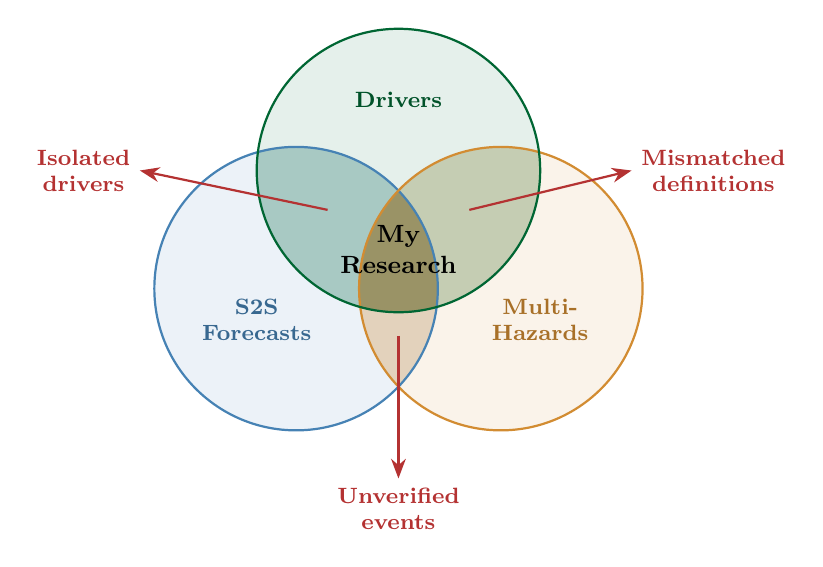
\begin{tikzpicture}
    \def\r{1.8}

    % Base circle fills
    \fill[vennblue!10] (-1.3,0) circle (\r);
    \fill[vennorange!10] ( 1.3,0) circle (\r);
    \fill[ucdgreen!10] (0,1.5) circle (\r);

    % Pairwise overlap fills (mixed colours)
    % Forecast ↔ Multi-Hazard (bottom)
    \begin{scope}
      \clip (-1.3,0) circle (\r);
      \clip ( 1.3,0) circle (\r);
      \fill[vennblue!25!vennorange, opacity=0.3] (-3,-3) rectangle (3,3);
    \end{scope}
    % Forecast ↔ Drivers (upper-left)
    \begin{scope}
      \clip (-1.3,0) circle (\r);
      \clip (0,1.5) circle (\r);
      \fill[vennblue!40!ucdgreen, opacity=0.3] (-3,-3) rectangle (3,3);
    \end{scope}
    % Drivers ↔ Multi-Hazard (upper-right)
    \begin{scope}
      \clip ( 1.3,0) circle (\r);
      \clip (0,1.5) circle (\r);
      \fill[ucdgreen!40!vennorange, opacity=0.3] (-3,-3) rectangle (3,3);
    \end{scope}

    % Triple intersection fill
    \begin{scope}
      \clip (-1.3,0) circle (\r);
      \clip ( 1.3,0) circle (\r);
      \clip (0,1.5) circle (\r);
      \fill[ucdgreen!30!vennblue!30!vennorange, opacity=0.5] (-3,-3) rectangle (3,3);
    \end{scope}

    % Circle outlines
    \draw[vennblue, thick] (-1.3,0) circle (\r);
    \draw[vennorange, thick] ( 1.3,0) circle (\r);
    \draw[ucdgreen, thick] (0,1.5) circle (\r);

    % Circle labels (inside, in non-overlapping region)
    \node[align=center, text=vennblue!80!black, font=\footnotesize\bfseries] at (-1.8,-0.4)
         {S2S\\Forecasts};
    \node[align=center, text=vennorange!80!black, font=\footnotesize\bfseries] at ( 1.8,-0.4)
         {Multi-\\Hazards};
    \node[align=center, text=ucdgreen!80!black, font=\footnotesize\bfseries] at (0,2.4)
         {Drivers};

    % Centre label (revealed on click)
    \onslide<2->{
    \node[align=center, font=\small\bfseries] at (0,0.5)
         {My\\Research};
    }

    % Gap labels with arrows from pairwise overlaps
    % Unverified: Forecast ↔ Multi-Hazard (bottom overlap → down)
    \node[align=center, font=\footnotesize\bfseries, text=gapred] (g1) at (0,-2.8)
         {Unverified\\events};
    \draw[-{Stealth[length=2.5mm]}, thick, gapred] (0,-0.6) -- (g1.north);

    % Isolated: Forecast ↔ Drivers (upper-left overlap → left)
    \node[align=center, font=\footnotesize\bfseries, text=gapred] (g2) at (-4.0,1.5)
         {Isolated\\drivers};
    \draw[-{Stealth[length=2.5mm]}, thick, gapred] (-0.9,1.0) -- (g2.east);

    % Mismatched: Drivers ↔ Multi-Hazard (upper-right overlap → right)
    \node[align=center, font=\footnotesize\bfseries, text=gapred] (g3) at (4.0,1.5)
         {Mismatched\\definitions};
    \draw[-{Stealth[length=2.5mm]}, thick, gapred] (0.9,1.0) -- (g3.west);

    \end{tikzpicture}
\end{frame}

% --------------------------------------------------
% SLIDE 5: Closing — restate core message
% --------------------------------------------------
\begin{frame}{}

    \vspace{1.5em}
    \begin{columns}[c,totalwidth=0.85\textwidth]

        \begin{column}{0.45\textwidth}
            \centering
            {\color{gapred}\Large\ding{55}}\\[0.5em]
            {\large\textbf{Current forecasts}}\\[0.8em]
            Hazards independent\\[0.3em]
            Relationships linear
        \end{column}

        \begin{column}{0.45\textwidth}
            \centering
            {\color{ucdgreen}\Large\ding{51}}\\[0.5em]
            {\large\textbf{Real-world risk}}\\[0.8em]
            Hazards connected\\[0.3em]
            Relationships nonlinear
        \end{column}

    \end{columns}

    \vspace{2em}
    \begin{center}
        \textit{When and where can S2S forecasts predict multi-hazard events?}
    \end{center}
\end{frame}

\end{document}
